\documentclass[11pt]{article}

\usepackage[margin=1in]{geometry}
\usepackage{graphicx}
\usepackage{array}
\usepackage{longtable}
\usepackage[hidelinks]{hyperref}

\newcommand{\state}[1]{\texttt{#1}}
\newcommand{\code}[1]{\texttt{#1}}
\setlength{\emergencystretch}{3em}

\title{ENSF 460 Project 1\\Countdown Timer Application}
\author{
    Group 06 -- Lecture Section L01\\[0.5em]
    David Burgoin -- UCID: 30214909 \\
    Moyo Ogunjobi -- UCID: \\
    Jacob Plourde -- UCID: 
}
\date{Fall 2026}

\begin{document}

\maketitle
\tableofcontents
\newpage

\section{Project Overview}

The project implements a countdown timer controlled by three push buttons and displayed on a PC terminal. The user can configure minutes and seconds, start the countdown, pause and resume it, clear it with a long press, and observe an alarm when the count reaches zero. The controller is implemented as a finite-state machine in \code{src/superloop.c}. This report documents the superloop and its state-dependent behavior.

\section{Superloop Architecture}

\subsection{Execution Model}

The application repeatedly calls \code{superloop\_loop()} from the infinite loop in \code{main()}. The superloop separates the active state, stored in \code{state}, from the next requested state, stored in \code{request\_state}. A transition requested during one iteration is applied at the beginning of the next iteration:

\begin{verbatim}
if (request_state != state)
{
    prev_state = state;
    state = request_state;
    counter = 0;
}
\end{verbatim}

This deferred-transition approach ensures that each state performs one well-defined set of actions per superloop iteration. It also prevents a chain of states from being executed in a single call.

The superloop uses the following shared variables:

\begin{longtable}{>{\ttfamily}p{0.28\textwidth}p{0.64\textwidth}}
\hline
\normalfont Variable & Purpose \\
\hline
\endhead
state & Current finite-state-machine state. \\
request\_state & State that will become active on the next iteration. \\
buttons & Push-button bit mask written by the CN interrupt service routine. \\
prev\_buttons & Previous button mask used to detect a changed combination. \\
counter & Number of repeated setting operations during a continuous hold. \\
preset\_mins & Configured countdown minutes. \\
preset\_secs & Configured countdown seconds. \\
elapsed\_value & Remaining countdown time represented in seconds. \\
elapsed\_before\_pause & Partial one-second interval saved when pausing. \\
selected\_message & Terminal message selected by the active state. \\
delay & Shared non-blocking delay object used by the state machine. \\
\hline
\end{longtable}
\pagebreak
\subsection{State Diagram}

\begin{figure}[htbp]
    \centering
    \IfFileExists{state_machine.png}{
        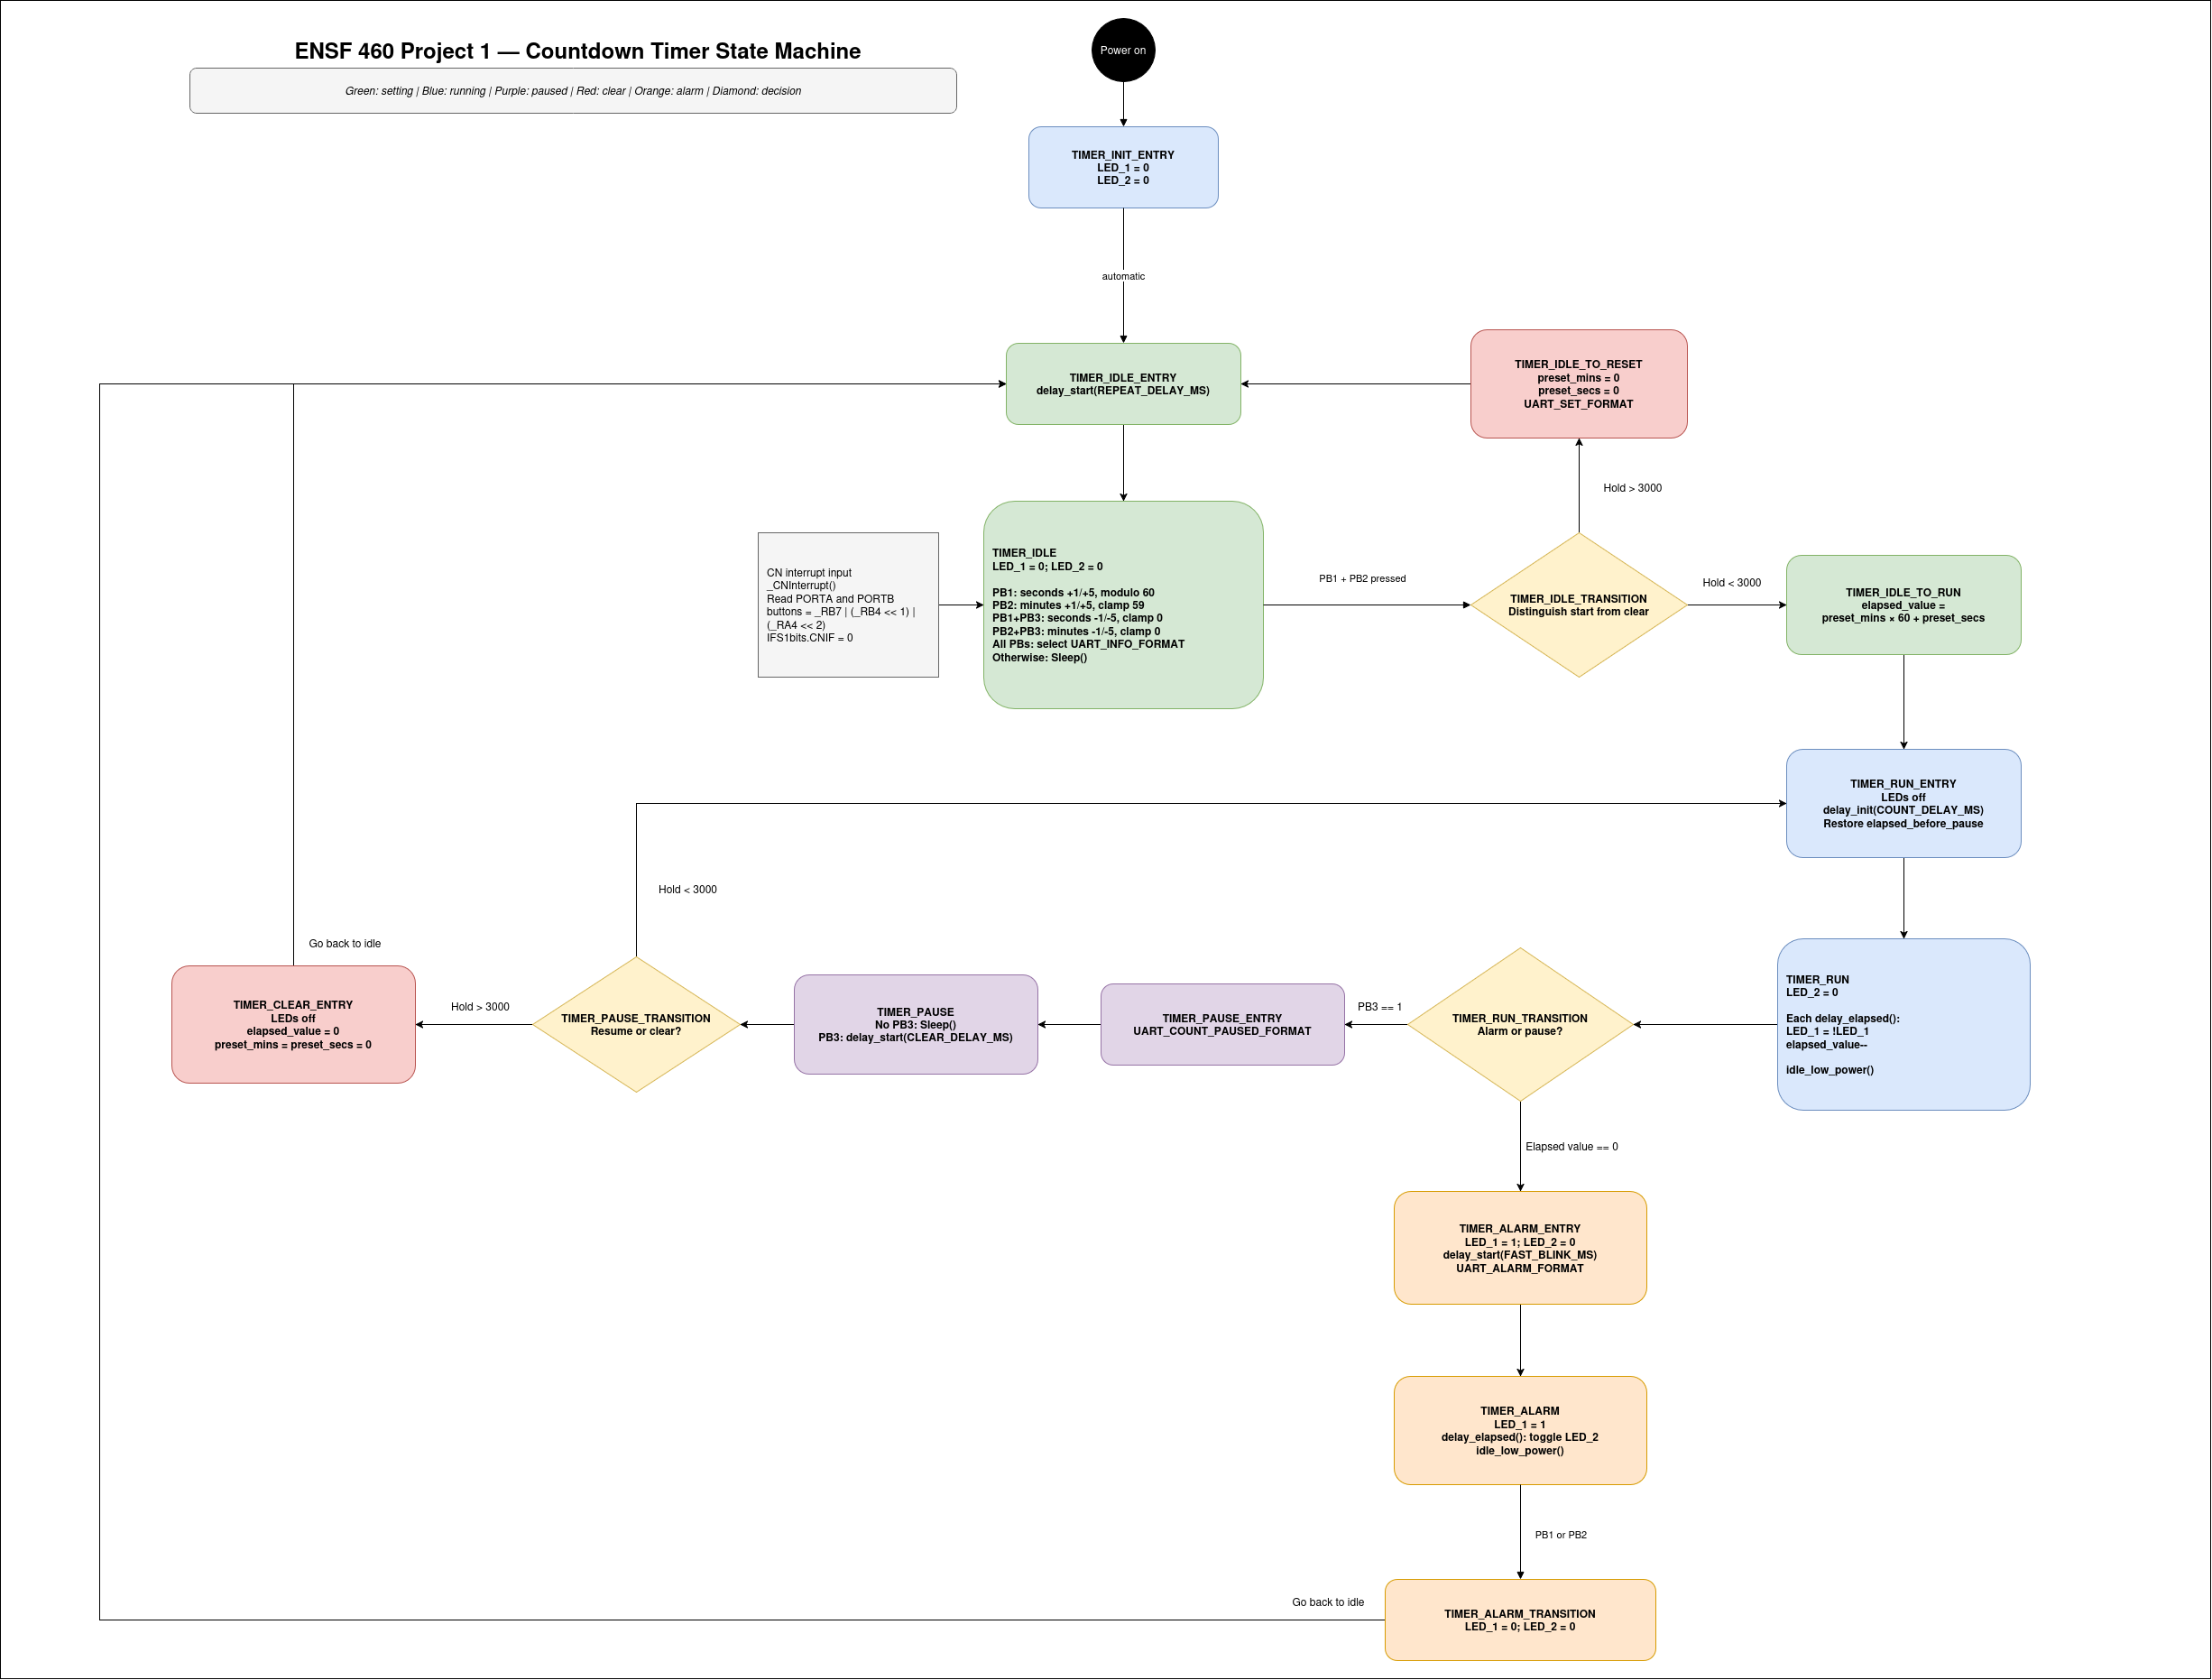
\includegraphics[width=\textwidth,height=0.78\textheight,keepaspectratio]{state_machine.png}
    }{
        \fbox{\parbox[c][5cm][c]{0.88\textwidth}{\centering
        Export \code{state\_machine.drawio} as \code{state\_machine.pdf} to place the diagram here.}}
    }
    \caption{Countdown timer finite-state machine.}
    \label{fig:fsm}
\end{figure}

\subsection{State Summary}

The implemented controller contains 17 active states. Entry states perform one-time setup, stable states perform repeated behavior, and transition states decide which state should execute next.

\begin{longtable}{>{\ttfamily}p{0.30\textwidth}p{0.62\textwidth}}
\hline
\normalfont State & Responsibility \\
\hline
\endhead
TIMER\_INIT\_ENTRY & Turns off both LEDs and requests idle initialization. \\
TIMER\_IDLE\_ENTRY & Starts the setting-repeat interval before entering idle. \\
TIMER\_IDLE & Processes setting controls and the three-button information command. \\
TIMER\_IDLE\_TRANSITION & Distinguishes a short start command from a held preset-clear command. \\
TIMER\_IDLE\_TO\_RUN & Converts the minute and second preset into total countdown seconds. \\
TIMER\_IDLE\_TO\_RESET & Clears the configured minutes and seconds. \\
TIMER\_RUN\_ENTRY & Initializes the one-second interval and restores a saved partial interval. \\
TIMER\_RUN & Decrements the timer, updates LED1, and detects completion or PB3. \\
TIMER\_RUN\_TRANSITION & Selects the alarm, pause, or clear path. \\
TIMER\_PAUSE\_ENTRY & Selects the paused countdown message. \\
TIMER\_PAUSE & Holds the countdown and waits for another PB3 press. \\
TIMER\_PAUSE\_TRANSITION & Distinguishes resume from a long-press clear. \\
TIMER\_CLEAR\_ENTRY & Clears the countdown, preset, and LED outputs. \\
TIMER\_CLEAR & Selects the clear message before returning to setting mode. \\
TIMER\_ALARM\_ENTRY & Enables the alarm indicators and selects the alarm message. \\
TIMER\_ALARM & Holds LED1 on, blinks LED2, and waits for a setting input. \\
TIMER\_ALARM\_TRANSITION & Turns off both LEDs and returns to setting mode. \\
\hline
\end{longtable}

\section{Push-Button Event Capture}

The push buttons are handled through the Change Notification peripheral rather than repeated reads of \code{PORTA} or \code{PORTB} in the superloop. The CN interrupt service routine first reads both ports to clear the hardware mismatch condition. It then packs the three button inputs into the shared \code{buttons} bit mask and clears \code{IFS1bits.CNIF}.

\begin{verbatim}
void __attribute__((interrupt, no_auto_psv)) _CNInterrupt(void)
{
    volatile uint16_t dummy_a = PORTA;
    volatile uint16_t dummy_b = PORTB;

    buttons = (uint16_t)_RB7
            | ((uint16_t)_RB4 << 1)
            | ((uint16_t)_RA4 << 2);

    (void)dummy_a;
    (void)dummy_b;
    IFS1bits.CNIF = 0;
}
\end{verbatim}

The interrupt routine contains no delay, UART output, loop, or function call. All state decisions are deferred to \code{superloop\_loop()}. The \code{volatile} qualifier on \code{buttons} informs the compiler that its value may change asynchronously.

The internal button enumeration represents every possible three-bit combination. This permits the idle state to select behavior with one \code{switch} statement instead of repeatedly reading hardware registers.

\section{Preset Configuration}

\subsection{Incrementing Minutes and Seconds}

While the timer is idle, holding PB1 increments \code{preset\_secs}, and holding PB2 increments \code{preset\_mins}. An adjustment occurs whenever \code{delay\_elapsed()} reports that the 500~ms repeat interval has completed. The setting therefore changes at a pace that permits the user to stop at a desired value.

The \code{counter} variable is incremented after every repeated adjustment. For the first ten adjustments, the value changes by one. After \code{INCREASE\_INCREMENT\_THRESHOLD} is exceeded, each adjustment changes the value by five:

\begin{verbatim}
counter++;
preset_secs += counter > INCREASE_INCREMENT_THRESHOLD ? 5 : 1;
preset_secs %= 60;
\end{verbatim}

The seconds value uses modulo 60 so a fast increment preserves its remainder when crossing 59. For example, a five-second increment from 58 produces 03. Minutes also support the fast increment, but are clamped at the maximum value of 59.

Whenever the button combination changes or the state machine enters a new state, \code{counter} is reset to zero. A new continuous hold therefore begins with single-unit adjustments before acceleration is enabled.

\subsection{Decrementing Minutes and Seconds}

PB3 acts as a decrement modifier while setting the timer. Holding PB1 with PB3 decreases seconds, while holding PB2 with PB3 decreases minutes. These combinations use the same repeat interval and the same transition from steps of one to steps of five. Both values are clamped at zero to prevent a negative preset.

\begin{verbatim}
preset_secs -= counter > INCREASE_INCREMENT_THRESHOLD ? 5 : 1;
preset_secs = preset_secs < 0 ? 0 : preset_secs;
\end{verbatim}

PB3 by itself is handled by the idle state's default path and does not modify the preset.

\subsection{Preset Display Selection}

Every successful preset adjustment selects \code{UART\_SET\_FORMAT}. The message is transmitted after state processing, keeping formatted output outside the interrupt service routine. Holding all three push buttons selects \code{UART\_INFO\_FORMAT}, which contains the course section and group number.
\pagebreak
\section{Starting and Resetting the Countdown}

PB1 and PB2 together are used for both starting and clearing the preset. When this combination is detected in \state{TIMER\_IDLE}, the controller starts the 3000~ms clear interval and requests \state{TIMER\_IDLE\_TRANSITION}.

If PB1 and PB2 are released before the interval expires and the preset is nonzero, the controller requests \state{TIMER\_IDLE\_TO\_RUN}. This state converts the preset into one total-second value:

\begin{verbatim}
elapsed_value = (uint16_t)(preset_mins * 60 + preset_secs);
\end{verbatim}

If the combination remains held for the complete interval, \state{TIMER\_IDLE\_TO\_RESET} clears both preset fields and returns to idle setup. If the buttons are released while the preset is 00:00, the controller returns to idle without starting a countdown. This explicitly handles the zero-length timer corner case.

\section{Running Countdown}

\state{TIMER\_RUN\_ENTRY} turns off both LEDs, configures the shared delay for the one-second countdown interval, and applies any partial interval saved before a pause. It then requests \state{TIMER\_RUN}.

While running, every completed interval toggles LED1 through the \code{LED\_1} macro, which maps to \code{\_LATB9}. If the remaining value is greater than zero, it is decremented exactly once:

\begin{verbatim}
if (delay_elapsed(&delay))
{
    LED_1 = !LED_1;
    if (elapsed_value > 0)
    {
        elapsed_value--;
    }
}
\end{verbatim}

The superloop compares \code{elapsed\_value} with \code{prev\_elapsed\_value}. A difference selects \code{UART\_COUNT\_FORMAT}, ensuring that the terminal count is updated when the displayed second changes rather than on every superloop iteration.

When \code{elapsed\_value} reaches zero, or when the PB3 bit becomes active, the running state saves the time already spent in the current one-second interval and requests \state{TIMER\_RUN\_TRANSITION}. The transition state sends a completed countdown to the alarm, a released PB3 to pause, or a PB3 held for 3000~ms to clear.

\section{Pause, Resume, and Long-Press Clear}

A short PB3 press while running leads to \state{TIMER\_PAUSE\_ENTRY}. This state selects the paused count message and then requests \state{TIMER\_PAUSE}. The countdown value is not decremented while paused.

Pressing PB3 again starts a new 3000~ms decision interval in \state{TIMER\_PAUSE\_TRANSITION}. Releasing PB3 before the interval expires requests \state{TIMER\_RUN\_ENTRY}, which resumes the countdown. Holding PB3 until the interval expires requests \state{TIMER\_CLEAR\_ENTRY}.

The partial interval saved in \code{elapsed\_before\_pause} prevents a pause and resume operation from discarding the portion of the current second that had already elapsed. On resume, the delay is enabled with an adjusted start value:

\begin{verbatim}
delay_enable(&delay, millis() - elapsed_before_pause);
elapsed_before_pause = 0;
\end{verbatim}

The clear entry state resets \code{elapsed\_value}, \code{preset\_mins}, and \code{preset\_secs}, turns off both LEDs, and enters \state{TIMER\_CLEAR}. The clear state selects \code{UART\_CLEAR\_FORMAT} before returning to idle setup.

\section{Alarm Behavior}

When the countdown reaches zero, \state{TIMER\_ALARM\_ENTRY} turns LED1 on, initializes LED2 to off, starts the 250~ms blink interval, and selects \code{UART\_ALARM\_FORMAT}. LED1 maps to \code{\_LATB9}, while LED2 maps to \code{\_LATA6}.

In \state{TIMER\_ALARM}, LED1 remains continuously on. Each completed fast-blink interval toggles LED2. Pressing either setting button requests \state{TIMER\_ALARM\_TRANSITION}, selects the preset display, turns both LEDs off, and returns the controller to idle setup.

\section{Terminal Message Selection}

The state machine does not print from any interrupt service routine. Instead, each state selects one member of \code{uart\_message\_e}. A single \code{switch} statement at the end of \code{superloop\_loop()} formats the selected message. \code{UART\_NONE} is selected at the start of every iteration so no output is produced unless the state machine explicitly requests it.

\begin{table}[htbp]
\centering
\begin{tabular}{ll}
\hline
Selection & Terminal content \\
\hline
\code{UART\_COUNT\_FORMAT} & Active countdown value \\
\code{UART\_COUNT\_PAUSED\_FORMAT} & Remaining value with a paused indicator \\
\code{UART\_ALARM\_FORMAT} & Finished value and alarm indicator \\
\code{UART\_SET\_FORMAT} & Configured minute and second preset \\
\code{UART\_INFO\_FORMAT} & Course section and group information \\
\code{UART\_CLEAR\_FORMAT} & Cleared 00:00 value \\
\hline
\end{tabular}
\caption{Messages selected by the superloop.}
\label{tab:messages}
\end{table}

\section{Corner Cases}

\begin{description}
    \item[Starting at 00:00:] Releasing PB1 and PB2 with a zero preset returns to idle instead of starting or immediately alarming.

    \item[Seconds above 59:] Incrementing seconds uses modulo 60, including when a five-second adjustment crosses the boundary.

    \item[Minutes above 59:] The minute preset is clamped at 59.

    \item[Decrement below zero:] Both minute and second decrement paths clamp their results at zero.

    \item[Countdown underflow:] The running state checks \code{elapsed\_value > 0} before decrementing.

    \item[Pause during a partial second:] The elapsed portion of the current interval is stored and restored when the countdown resumes.

    \item[Arbitrary button combinations:] The complete three-bit button enumeration gives each recognized combination an explicit setting behavior or routes it through the default path.

    \item[Invalid state value:] The default state-machine branch requests \state{TIMER\_INIT\_ENTRY}, allowing the controller to return to a known state.

    \item[Alarm dismissal:] PB1 or PB2 turns off both alarm LEDs and restores the preset display.
\end{description}



\section{UART}

\section{Timer}

\section{Power Management}

\subsection{Low-Power Features in the Test Firmware}

Several complementary power-saving techniques were added to the test firmware before the measurements were collected. Unused peripheral modules are disabled through the Peripheral Module Disable registers. Push-button activity and elapsed time are detected with Change Notification and timer interrupts so the processor does not need to poll the input ports or timer registers. When the processor is waiting, the superloop enters either \code{Idle()} or \code{Sleep()} instead of executing a busy loop. Before entering these modes, UART2 is allowed to finish its current transmission and is then shut down. The UART is only enabled again when a new message must be sent, and messages are suppressed when the displayed value has not changed. For the \code{Idle()} path, the system clock is temporarily switched to the low-power 32~kHz oscillator and is restored after an interrupt wakes the processor. The timer and UART drivers are reconfigured whenever the system clock changes so that timing and communication remain correct. Together, peripheral gating, interrupt-driven operation, low-power CPU modes, dynamic clock scaling, UART duty cycling, and output-on-change messaging reduce the time for which the CPU and peripherals remain fully active.

\subsection{Power-Test Methodology}

Power consumption was investigated by operating the microcontroller at several clock frequencies and supply voltages. The tested clock settings were 31~kHz, 500~kHz, 1~MHz, 4~MHz, 8~MHz, and 32~MHz. The lowest-frequency setting is rounded to 32~kHz in the firmware constants. Each clock setting was tested at supply voltages of 1.8~V, 2.4~V, 3.0~V, and 3.3~V. This produced a test matrix of 24 frequency-and-voltage combinations, with two automated usage profiles attempted for each combination. The purpose of these tests was to determine how far the clock frequency and supply voltage could be reduced while preserving correct timer, push-button, LED, and UART operation. The voltage was adjusted externally; it is therefore not selected by the firmware.

The two profiles were scripts from the hardware-in-the-loop test harness. Test~03, \code{power\_short\_run\_alarm\_dwell}, was the more active workload. It configured and started two short countdowns, allowed each countdown to finish, remained in the alarm state for extended periods, and dismissed the alarms using the setting buttons. This profile repeatedly exercised countdown timing, UART updates, LED1 blinking, and the rapid LED2 alarm blink, with only brief idle intervals between operations.

Test~04, \code{power\_idle\_preset\_fiddling}, represented a mostly idle or sleeping workload. It did not start the countdown. Instead, it left the controller in the preset-setting state, separated short button operations with waiting intervals, and adjusted the seconds and minutes in both directions. The profile also held each setting combination for ten seconds to exercise button auto-repeat and accelerated adjustment. Between button events the processor could enter \code{Sleep()}, while during a held button it repeatedly returned to the low-frequency \code{Idle()} path. Test~04 therefore measured a usage pattern dominated by low-power waiting, with brief wakeups for Change Notification interrupts, preset calculations, and UART output. Table~\ref{tab:power-results} gives the measured average current for both profiles in microamperes.

\begin{table}[htbp]
\centering
\small
\setlength{\tabcolsep}{4pt}
\begin{tabular}{l*{8}{c}}
\hline
& \multicolumn{2}{c}{1.8~V} & \multicolumn{2}{c}{2.4~V} & \multicolumn{2}{c}{3.0~V} & \multicolumn{2}{c}{3.3~V} \\
Clock & 03 & 04 & 03 & 04 & 03 & 04 & 03 & 04 \\
\hline
31~kHz  & X           & X           & X    & X    & 16.9 & 24.1 & 19.3 & 27.3 \\
500~kHz & 16.4        & 17.4        & 19.8 & 20.1 & 20.7 & 21.5 & 24.1 & 25.7 \\
1~MHz   & 20.1        & 21.8        & 25.9 & 24.1 & 28.1 & 27.2 & 36.6 & 30.9 \\
4~MHz   & 29.4        & 28.7        & 30.9 & 30.2 & 33.2 & 34.4 & 56.4 & 42.4 \\
8~MHz   & 34.0$^{*}$  & 29.7$^{*}$  & 40.6 & 25.2 & 79.4 & 40.3 & 90.5 & 57.9 \\
32~MHz  & 20.9$^{*}$  & 18.1$^{*}$  & 29.4 & 26.0 & 35.3 & 29.1 & 57.3 & 37.6 \\
\hline
\end{tabular}
\caption{Measured average current in $\mu$A for power-profiling Tests 03 and 04. An X indicates that the configuration failed the test. An asterisk marks a measurement taken outside the device's specified operating range.}
\label{tab:power-results}
\end{table}

\subsection{Results and Observations}

The measurements generally show that reducing the supply voltage and clock frequency reduced average current. The lowest result from a configuration within its specified operating range was 16.4~$\mu$A for Test~03 at 500~kHz and 1.8~V. At 3.0~V, where every clock setting passed both profiles, the 31~kHz configuration measured 16.9~$\mu$A in Test~03 and 24.1~$\mu$A in Test~04. The 31~kHz configuration failed both profiles at 1.8 and 2.4~V. The 8 and 32~MHz measurements at 1.8~V are marked with an asterisk because these clock rates require a minimum supply of approximately 2.4~V. Although current readings were obtained, these four points were outside the specified operating range and were excluded when identifying the lowest valid result. The profile also affected the average because Test~03 repeatedly runs the countdown and alarm outputs, whereas Test~04 remains in preset mode and spends most of its duration waiting in \code{Idle()} or \code{Sleep()}. Consequently, readings from the two test columns describe different workloads and should not be treated as repeat measurements of an identical sequence. The non-monotonic results at the higher clock settings also show that clock frequency alone does not determine the average: completing active work more quickly and returning to a low-power mode can offset some of the higher instantaneous current of a faster clock.

\subsection{Clock and Peripheral Management}

The clock selections are represented by the \code{core\_clock\_freq\_e} enumeration and are applied by \code{set\_core\_clock()}. This function switches the oscillator source and, when required, changes the FRC divider. The 32~MHz setting uses the FRC oscillator with the PLL, the 8, 4, and 1~MHz settings use divided FRC clock configurations, the 500~kHz setting uses the low-power FRC oscillator, and the lowest-frequency test uses the approximately 32~kHz low-power oscillator. Before a clock change, the code waits for any UART transmission to finish and temporarily raises the CPU interrupt priority level. It then stops the active timers, performs the oscillator switch, waits for the switch and PLL to become ready, and reconfigures the timer and UART drivers for the new clock frequency. These steps prevent a partially transmitted message or a timer interrupt during the transition from producing incorrect behavior.

The firmware also reduces the number of powered peripherals. During \code{superloop\_setup()}, the Peripheral Module Disable registers turn off hardware that is not required by this application, including the ADC, SPI1, UART1, I2C1, Timer1, Output Compare 1, Input Capture 1, CRC, RTCC, comparator, high/low-voltage detect, CTMU, reference oscillator, and EEPROM modules. UART2, the Change Notification peripheral, and the timer required for the current clock mode remain available because they are needed by the application.

\subsection{Idle and Sleep Operation}

Two low-power paths were tested in the superloop. The \code{IDLE\_LOW\_POWER()} macro first shuts down UART2, changes the system clock to the low-power 32~kHz setting, and executes \code{Idle()}. An interrupt wakes the processor, after which the macro restores the selected normal test frequency. This path is used while the preset button is being held, while the countdown is running, and while the alarm is active. The \code{SLEEP\_WHEN\_UART\_IDLE()} macro waits until UART output is complete, disables UART2, and executes \code{Sleep()}. It is used when the timer is waiting with no setting input and while the countdown is paused. A Change Notification interrupt from a push button can wake the device. UART2 is re-enabled automatically by \code{uart\_wake()} when the next terminal message must be sent, so it does not remain powered solely while the program is waiting.

\subsection{Timer and UART Scaling}

Maintaining timing accuracy at every tested frequency required two timer configurations. At clock frequencies from 500~kHz through 32~MHz, Timer3 provides the millisecond time base and its prescaler and period are updated for the active clock. At the lowest-frequency setting, Timer3 is stopped and Timer2 supplies the time base instead. The timer driver stops and resets the appropriate timer before every clock transition and starts the correct timer afterward. This allows the state machine to continue using the same non-blocking elapsed-time calculations for button-repeat intervals, the three-second long-press interval, the one-second countdown, and the alarm blink interval.

The UART baud rate was also reduced with clock frequency. The test firmware uses 500000~baud at 4, 8, and 32~MHz, 125000~baud at 1~MHz, 62500~baud at 500~kHz, and 300~baud at approximately 32~kHz. The baud-rate generator value is recalculated from the current instruction clock whenever the clock changes. Terminal messages are only sent when the state or displayed value changes, and UART2 is shut down between required transmissions. Together, clock reduction, peripheral gating, low-power CPU modes, and limited UART activity were the principal techniques evaluated to reduce power consumption.

\section{Conclusion}

The superloop implements the countdown timer as a finite-state machine with separate entry, stable, and decision states. Button events are captured by the CN interrupt and processed outside the ISR. The state logic covers preset adjustment, accelerated changes, starting, preset reset, countdown operation, pause and resume, long-press clear, alarm behavior, LED control, message selection, and boundary conditions.

\end{document}
